\appendix



\chapter{Source Selection and Analysis Method: Non-Functional Requirements for
Service-Based Applications}
\label{append:analysis}


We selected the sources proposed by \cite{Kitchenham08} for searching primary
studies. These sources contain the works published in journals, conferences and
workshops which are of recognized quality within the research community. The
search for bibliography was performed in the engines are: \textit{(i) IEEE
Computer; (ii) ACM Digital Library;} and \textit{(iii) Science Direct}. For each
of the the selected sources, we used the following search query criteria:

\begin{center}
\texttt{(((``non functional properties'') OR (``non functional requirements''))
AND ``web service'' AND ``composition''))}
\end{center}

   
After define the sources' selection, we identify those works that provided direct
evidence with regard to the research questions. Deciding
for the inclusion and exclusion criteria for filtering the corpus works
selection, we selected those related to non-functional requirements/properties,
and quality for web service based applications. Initially, the selection
criteria were interpreted liberally and clear exclusions were only made with
regard to title, abstract and introduction.

Based on the guidelines mentioned in \cite{Kitchenham08}, we established a
three-step with different selection criteria:

\begin{itemize}
\item Step 1 - the search string must be run on the selected
search engine. An initial set of studies was obtained by filtering
of title, abstract, and if necessary, introduction. All the studies were
selected according to the inclusion and exclusion criteria. Studies which
were not clearly related to any aspect of the research questions
were excluded.
\item Step 2, the exclusion criteria were based on the following
practical issues: non-English papers, non-
International Conference papers and non-International Workshop
papers. Specifically in the case of ACM library, we considered only the
transaction journal works.
\item Step 3, the papers selection process was based on detailed
research questions ($RQ_1$ to $RQ_7$).
\end{itemize}

The information for each step was collected considering the 3 searchers
and the the query presented previously. the results of each step were:
\textit{(i)} for each source a list of all the studies that
fulfilled the query; \textit{(ii)} a list
of studies for each source which contained all the works that did not fulfill the
second stage inclusion criteria; and
\textit{(iii)} the last step produced a list of works for each source which
contained all the studies that fulfilled the second step (table
\ref{tab:result01}).

 
\begin{table}
\begin{tabular}{l|c|c|c|c}
  \hline
  \hline
   & IEEE Explorer & ACM Library & Science Direct & Total \\
  \hline
  \hline
  Total results & 65 & 271 (75 \footnote{We considered only 75 transactions
  journal works}) & 166 & 502 (306 \footnote{considering the 75 ACM
  transactions journal works}) \\ 
  \hline
  Step one - results selected & 19 & 10 & 20  & 49 \\
  Step one - results selected (\%) & 29.23\% & 13.33\% & 12\% &
  16\% \\ 
  \hline 
  Step two - results selected & 7 & 3 & 9 & 19\\
  Step two - results selected (\%)  & 10.76\% & 4\% & 5.42\% & 6.20\%\\ 
  \hline
  \hline
\end{tabular}
\caption{Summary of the studies selected at each step.}
\label{tab:result01}
\end{table} 

 
The extraction of information was based on the research questions, and each work extraction question included the following
items: \textit{(i)} where the paper was found; \textit{(ii)} identification of the title and main
subjects; \textit{(iii)} summary of the research; \textit{(iv)} inclusion and
exclusion criteria; \textit{(v)} objective and result; and \textit{(vi)}
subjective results.

% The systematic literature review took place between December 2011 and January
% 2012 and we did not filter works within a specific year interval. Although the
% studies which were concretely analyzed were published between 2005 and 2011.
Table \ref{tab:result01} shows a summary of the studies selected in each stage
of the selection procedure for each source. The ``Total results'' were obtained
by running the search string on the selected sources. The next four rows show
the results obtained after applying stages one (2 first rows) and two (2 last
rows) of the studies selection procedure. 

In the first step, respecting the filters described, the 65 articles collected
from IEEE, only 29.23\% of them were in accordance with the criteria
described early, representing 19 articles. In ACM Library, from 75 works
collected, only 13.33\% passed in the first stage filter, representing 10 articles. In Science Direct
had the lowest percentage, totaling 20 of the 166 articles collected by the
query, thus representing 12\% of the total. Despite being the lowest relative
value, the Science Direct had the largest absolute result, with 20 works
in the first step. In the second stage, the percentage dropped further, and the
relevant works and with accordance to the criteria have been collected as the
final result. The results were respectively, 10.76\%, 4\% and 5.42\% of total
from the IEEE, ACM and Science Direct. The highest percentage was among the
 works from  IEEE, while the largest number od results, in absolute terms,
 was collected from Science Direct. The approaches resulting from this last
 stage were studied in depth and information concerning the detailed research
 questions and other fields of the extraction forms was extracted from each
 eork we selected. 49 works were selected in the first stage, and, only 19
 works in the second stage. It represents  6.20\% of the total amount of works.

Figure \ref{fig:statistics} shows the publications per year, from
2005 to 2011. 12 of 19 articles were selected in the systematic review published
in 2006, 2009 and 2010, being four in each year and 6 in Science Direct source,
5 in IEEE, and only 1 at the ACM. All nine of Science Direct were
published in the last 4 years. Figure also
shows that the number of publications that consider classification of NFR once
again increased from 2008. 

\begin{figure} 
\centering
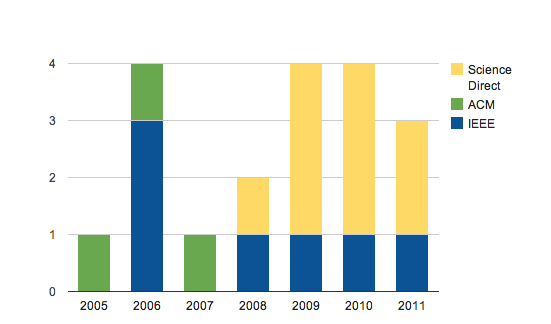
\includegraphics[width=.6\textwidth]{chapters/state_ofthe_art/figs/data.png}
\caption{Publications per year.}
\label{fig:statistics}
\end{figure} 


%%%%%%%%%%%%%%%%%%%%%%% APENDICE %%%%%%%%%%%%%%%%%%%%
%%%%%%%%%%%%%%%%%%%%%%% APENDICE %%%%%%%%%%%%%%%%%%%%
%%%%%%%%%%%%%%%%%%%%%%% APENDICE %%%%%%%%%%%%%%%%%%%%


\chapter{Service-Based Non-Functional Requirement Concepts}
\label{app:nfr-concepts}

\begin{itemize} 
  \item \textsc{Non-Functional (NF) Attribute -} An attribute that describes
the quality or characteristics of a functional requirement. For example
\textit{confidentiality} and \textit{privacy} may be
non-functional attributes for the functional requirement \textit{user
registration}.
  \item \textsc{Non-Functional (NF) Requirement -} A group of semantically
correlated non-functional attributes (NFA). For example, \textit{security} is
an NF Requirement that comprises attributes such as \textit{confidentiality}
and \textit{integrity}. 
  \item \textsc{Constraint -} A constraint prevents the system
  from achieving more than its goal. With the definition of constraints, the
  system  can be more robust, and unexpected problems can be solved before they
  happen. For example, in a banking system, the customer can only withdraw
  money if they have positive balance in the account.
    \item \textsc{Constraint Type -} Represents the types of
  constraints that could be expressed, the types are: business and data
  (*value) constraints. When modeling a system requirement the analyst can identify if there are restrictions on
  business, or data, or both. 
  \item \textsc{Contract -} Is the formalization of obligations (requires) and
  benefits (ensures) of a function, service activity or component.
  The following questions can be used to define contracts: \textit{What does it
  expect? What does it guarantee?} Contract can be crucial to software
  correctness that they should be part of the design process.
  \item \textsc{Exceptional Behaviour -} Are alternative execution paths if
  any condition or restriction is not respected. For example, if a user's password
  is not correct after three attempts, the user's account is locked for
  security.
  \item \textsc{Policy -} A policy is a set of rules applied to a particular
  scope. This scope can be defined as an action, an activity, a function or a
  workflow. A policy is a composition of contracts applied to a non-functional
  application requirement. For example, a security policy of a system constraint
  includes authentication, access, data privacy, and so on.
 \item \textsc{Use Case -} Represents a behavior that can be executed
in order to realize (parts of) a functional requirement.
%   \item \texttt{Composite Use Case -} Represents a set of actions performed by
%   the system to carry out part of a business service, which can be broken down
%   into different use cases, which may in turn be basic or composite.
  \item \textsc{Requirement -} A requirement is a super type for functional and
  non-functional requirements. Thus, the use cases can be related to both types
  of requirements.
  \item \textsc{Service Activity -} Represents a function of a software
  system or its component that are implemented through services. A Service
  Activity may be calculations, technical details, data manipulation and
  processing and other specific functionality that are available to be accessed
  on the Internet.
  \end{itemize}

%%%%%%%%%%%%%%%%%%%%%%% APENDICE %%%%%%%%%%%%%%%%%%%%
%%%%%%%%%%%%%%%%%%%%%%% APENDICE %%%%%%%%%%%%%%%%%%%%
%%%%%%%%%%%%%%%%%%%%%%% APENDICE %%%%%%%%%%%%%%%%%%%%

\chapter{\textit{$\pi$-PEWS} Language}
\label{append:pews_language}


$\pi$-PEWS specifies assertions that are checked during the execution of
a program. These assertions describe pre- and post-conditions for a given
operation or compound service. In the case these conditions are not verified,
the contract defines correcting actions (described as a PEWS path expression).
%
%Works try to adapt some tools and
%approaches aiming add quality constraints, like \textit{Behavioral Specification
%Language}, such as: Eiffel~\cite{Meyer98a}, JML~\cite{burdy:05}, JCML~\cite{jcml09} and
%IContract~\cite{LacknerKP02}, \textit{Graph Transformation}
%\cite{HL05TACoS, LeS92} and \textit{Transaction Specification Definition}
%\cite{PiresBM02, Hernandez-BaruchPZ07, Haddad08} for service composition.
%However, none of than proposes a hole application of service composition and
%behavioral specification definition for web services. 
%
The grammar defining the new language is defined as follows:
A $\pi$-PEWS program is similar to a PEWS program, but with the possibility of adding contract definitions at the end of the program.
Path expressions, defining the service workflow, are described by the \textit{Service} non-terminal of the grammar below. 
Since contracts and workflow are separate concerns, the syntax of path expressions remain unchanged, from the original version of the language.
\begin{small}
%\hrule
\begin{tabbing}
\reg \textit{Program} ::=\=  \ $\ldbrack\ ($``$\mathbf{var}$''$\ \mathbf{id}\ $``$=$''$ \mathit{ArithExp} )^*  \ ($``$\mathbf{service}$''$\ \mathbf{id}\ $``$=$''$ \mathit{Service})^* %$ \\ \> $
                                               %\qquad 
                                               \mathit{Service}\ \mathit{Contract}^ *\ \rdbrack$\\[1.5mm] 
\reg \textit{Service} ::=\=  \ $\ 	\ \ldbrack\  \mathbf{id} \ \rdbrack\ 
                                              \mid\ \ldbrack\ \mathit{Service}\ $``$.$''$\ \mathit{Service} \ \rdbrack\ 
                                              \mid\ \ldbrack\ \mathit{Service} $``$+$''$\ \mathit{Service} \ \rdbrack\ 
                                              \mid\ \ldbrack\  \mathit{Service} $``$\|$''$\ \mathit{Service} \ \rdbrack\ $\\ \>$
                                              \mid\ \ldbrack\  \mathit{Service}$``$*$''$\ \rdbrack\ 
                                              \mid\ \ldbrack\ $``$[$''$\ \mathit{BooleanCondition}\ $``$]$''$ \ \mathit{Service}\ \rdbrack\ 
                                              \mid\ \ldbrack\ $``$\{$''$\ 
                                              \mathit{Service}\ $``$\}$''$ \
                                              \rdbrack\ $\\[-3mm]
\end{tabbing}
\end{small}
%\hrule
%\vspace*{2mm}

The definition of contracts is given below. 
It includes a name for the contract, as well as its four component sections:
\begin{trivlist}
\item[$\bullet$] Target service of the contract: This section specifies the service to which the contract applies. This can be an operation or a compound service (which also defines a scope for the contract).
\item[$\bullet$]Preconditions and their actions. This section defines the assertions that will be verified before the target service is executed. 
\item[$\bullet$] Post-conditions and their actions. This section defines the assertions that will be verified at the end of the target service execution. 
\item[$\bullet$] Time constraints for the services on the contract scope.
\end{trivlist} 

%\bigskip

%\hrule
\begin{small}
\begin{tabbing}
\reg \textit{Contract} ::= \= $\ldbrack$ ``\textbf{def}'' ``\textbf{Contract}'' 
 \textit{Id} ``\textbf{\{}'' 
    \textit{IsAppliedTo}  
  \textit{Requires*}
  \textit{Ensures*} %\\
%\> \qquad\qquad\qquad\qquad\qquad\qquad\qquad\qquad\qquad   
\textit{(TimeConstraint)?} ``\textbf{\}}'' $\rdbrack$ \\[-3mm]
\end{tabbing}
%\hrule
%\vspace*{2mm}
\end{small}

The directive ``\textbf{isAppliedTo:}'' defines the target service and scope of the contract. 
This service is given by the identifier appearing next to the keyword.
The target service can be a simple operation or a compound service. 
In the former case, the contract cannot contain any time restriction.
In the case of a contract defined for a compound service, the operations and services that form the contract can participate of the time constraint expressions defined by the contract. %\nopagebreak\\
%\hrule
\begin{small}
\begin{tabbing}
 \reg \textit{isAppliedTo} ::= \= $\ldbrack$ ``\textbf{isAppliedTo}''
  ``\textbf{:}''  \textit{ident} ``\textbf{;}'' $\rdbrack$ \\[-3mm]
  \end{tabbing}
%\hrule
%\vspace*{2mm}
\end{small}

The ``\textbf{requires}'' and ``\textbf{ensures}'' parts of a contract define the pre-conditions (resp. post-conditions) to be checked for each contract. 
In the case of pre-conditions, they will be verified before the service is executed.
Post-conditions will be checked after the execution of the service.
In both cases, when the assertion fails, the associated action will be executed.
Actions are defined as services, and written as PEWS path expressions.
%\\
%\hrule
\begin{small} 
\begin{tabbing}
\reg \textit{Requires} ::= \= $\ldbrack$ ``\textbf{requires}''
  \textit{BooleanCondition} \textit{(} ``\textbf{(}'' \textit{onFailureDo} ``\textbf{)}''
  \textit{)?} ``\textbf{;}'' $\rdbrack$
  \\[1.5mm]
   
   \reg \textit{ensures} ::= \= $\ldbrack$ \textbf{`ensures'}
  \textit{BooleanCondition} \textit{(} ``\textbf{(}'' \textit{onFailureDo} ``\textbf{)}''
    \textit{)?} ``\textbf{;}'' $\rdbrack$
  \\[1.5mm]
  
   \reg \textit{onFailureDo} ::= \= $\ldbrack$ \textbf{`onFailureDo'}
  \textit{Service} $\rdbrack$ \\[-3mm]
\end{tabbing}
%\hrule 
%\vspace*{2mm}
\end{small}

Time Constraints are defined as relational expressions build from the operators.
%These constraints will be imposed to the execution of the composition.
%\hrule
\begin{small} 
\begin{tabbing}
  \reg \textit{timeConstraint} ::= \= $\ldbrack$ \textbf{`timeConstraint'} \textbf{`:'} 
                                                   ($\ldbrack$  ``\textbf{meet}'' $\rdbrack$ $|$ $\ldbrack$  ``\textbf{start}'' $\rdbrack$ $|$
                                                    $\ldbrack$  ``\textbf{overlap}'' $\rdbrack$) \\ \>
%  \textit{timeRelation} 
  \textbf{`('} 
  (\textit{opName} $|$ \textit{timeConstraint}) 
  \textbf{`,'} (\textit{opName} $|$ \textit{timeConstraint}) \textbf{`)'} $\rdbrack$ 

\end{tabbing}
%\hrule
%\vspace*{2mm}
\end{small} 

The model of temporal relations proposed here follows the main ideas presented in
\cite{Allen:1983, BeVaC00}. The model is used to impose additional restrictions
to the order in which operations of a web service are performed at execution time. For example, the
confirmation of the bank authorization request must arrive at most one minute after the service call.
 
A service composition time relation is represented by the following
model: Let   $\Omega$ be a set of web services ($\omega_1$, . . .,
$\omega_n$) to be composed and $\Theta$, a set of temporal relations $r_t$ that can be applied to $\Omega$. 
Temporal relations are defined by predicates $r_t:\ \Omega$ x $\Omega$, where
$r_t \in~\{\textbf{\textit{ %none, 
%before, 
meet, overlap, start
%, during, finish, equal
}}\}. $

For example, the  
%following expression defines that the operation $\omega_1$ needs to be finished before the operation $\omega_3$ is allowed to start: 
%\textbf{\textit{before($\omega_1, \omega_3$)}}.  
%The 
expression \textbf{\textit{meet($\omega_1, \omega_2$)}}
states that the execution of operation $\omega_2$ will begin as soon as $\omega_1$ finishes.
The temporal relations are described below:



\begin{trivlist}

%_._..__._..__._..__._..__._..__._..__._..__._..__._..__._..__._..__._..__._..__._.._
\item{\bf\em Meet.}
%_._..__._..__._..__._..__._..__._..__._..__._..__._..__._..__._..__._..__._..__._.._
The restriction specified by \textbf{\textit{meet($\omega_1, \omega_2$)}} specifies that $\omega_2$ will be executed immediately after $\omega_1$ finishes.

%_._..__._..__._..__._..__._..__._..__._..__._..__._..__._..__._..__._..__._..__._.._
\item{\bf\em Overlap.}
%_._..__._..__._..__._..__._..__._..__._..__._..__._..__._..__._..__._..__._..__._.._
The constraint given by \textbf{\textit{overlap($\omega_1, \omega_2$)}}
%,  shown in Figure~\ref{graph:overlap}, 
states that execution of the two services overlap in time. 
The restriction also states that the service $\omega_1$ initiates before $\omega_2$.
  
%_._..__._..__._..__._..__._..__._..__._..__._..__._..__._..__._..__._..__._..__._.._
\item{\bf\em Start.}
%_._..__._..__._..__._..__._..__._..__._..__._..__._..__._..__._..__._..__._..__._.._
The specification of \textbf{\textit{start($\omega_1, \omega_2$)}}
%, shown in Figure~\ref{graph:start}, 
states that the two services have their execution in parallel and that they start at the same time. 

\end{trivlist} 
  
% Considering the example scenario, the $\pi$-PEWS code generated from the
% $\pi$-PEWS model is describe as following\ldots 
  

\chapter{\textit{To Publish Music} Case Study Diagrams}
\label{append:diagrams}
  

\begin{figure}[ht!]
\centering
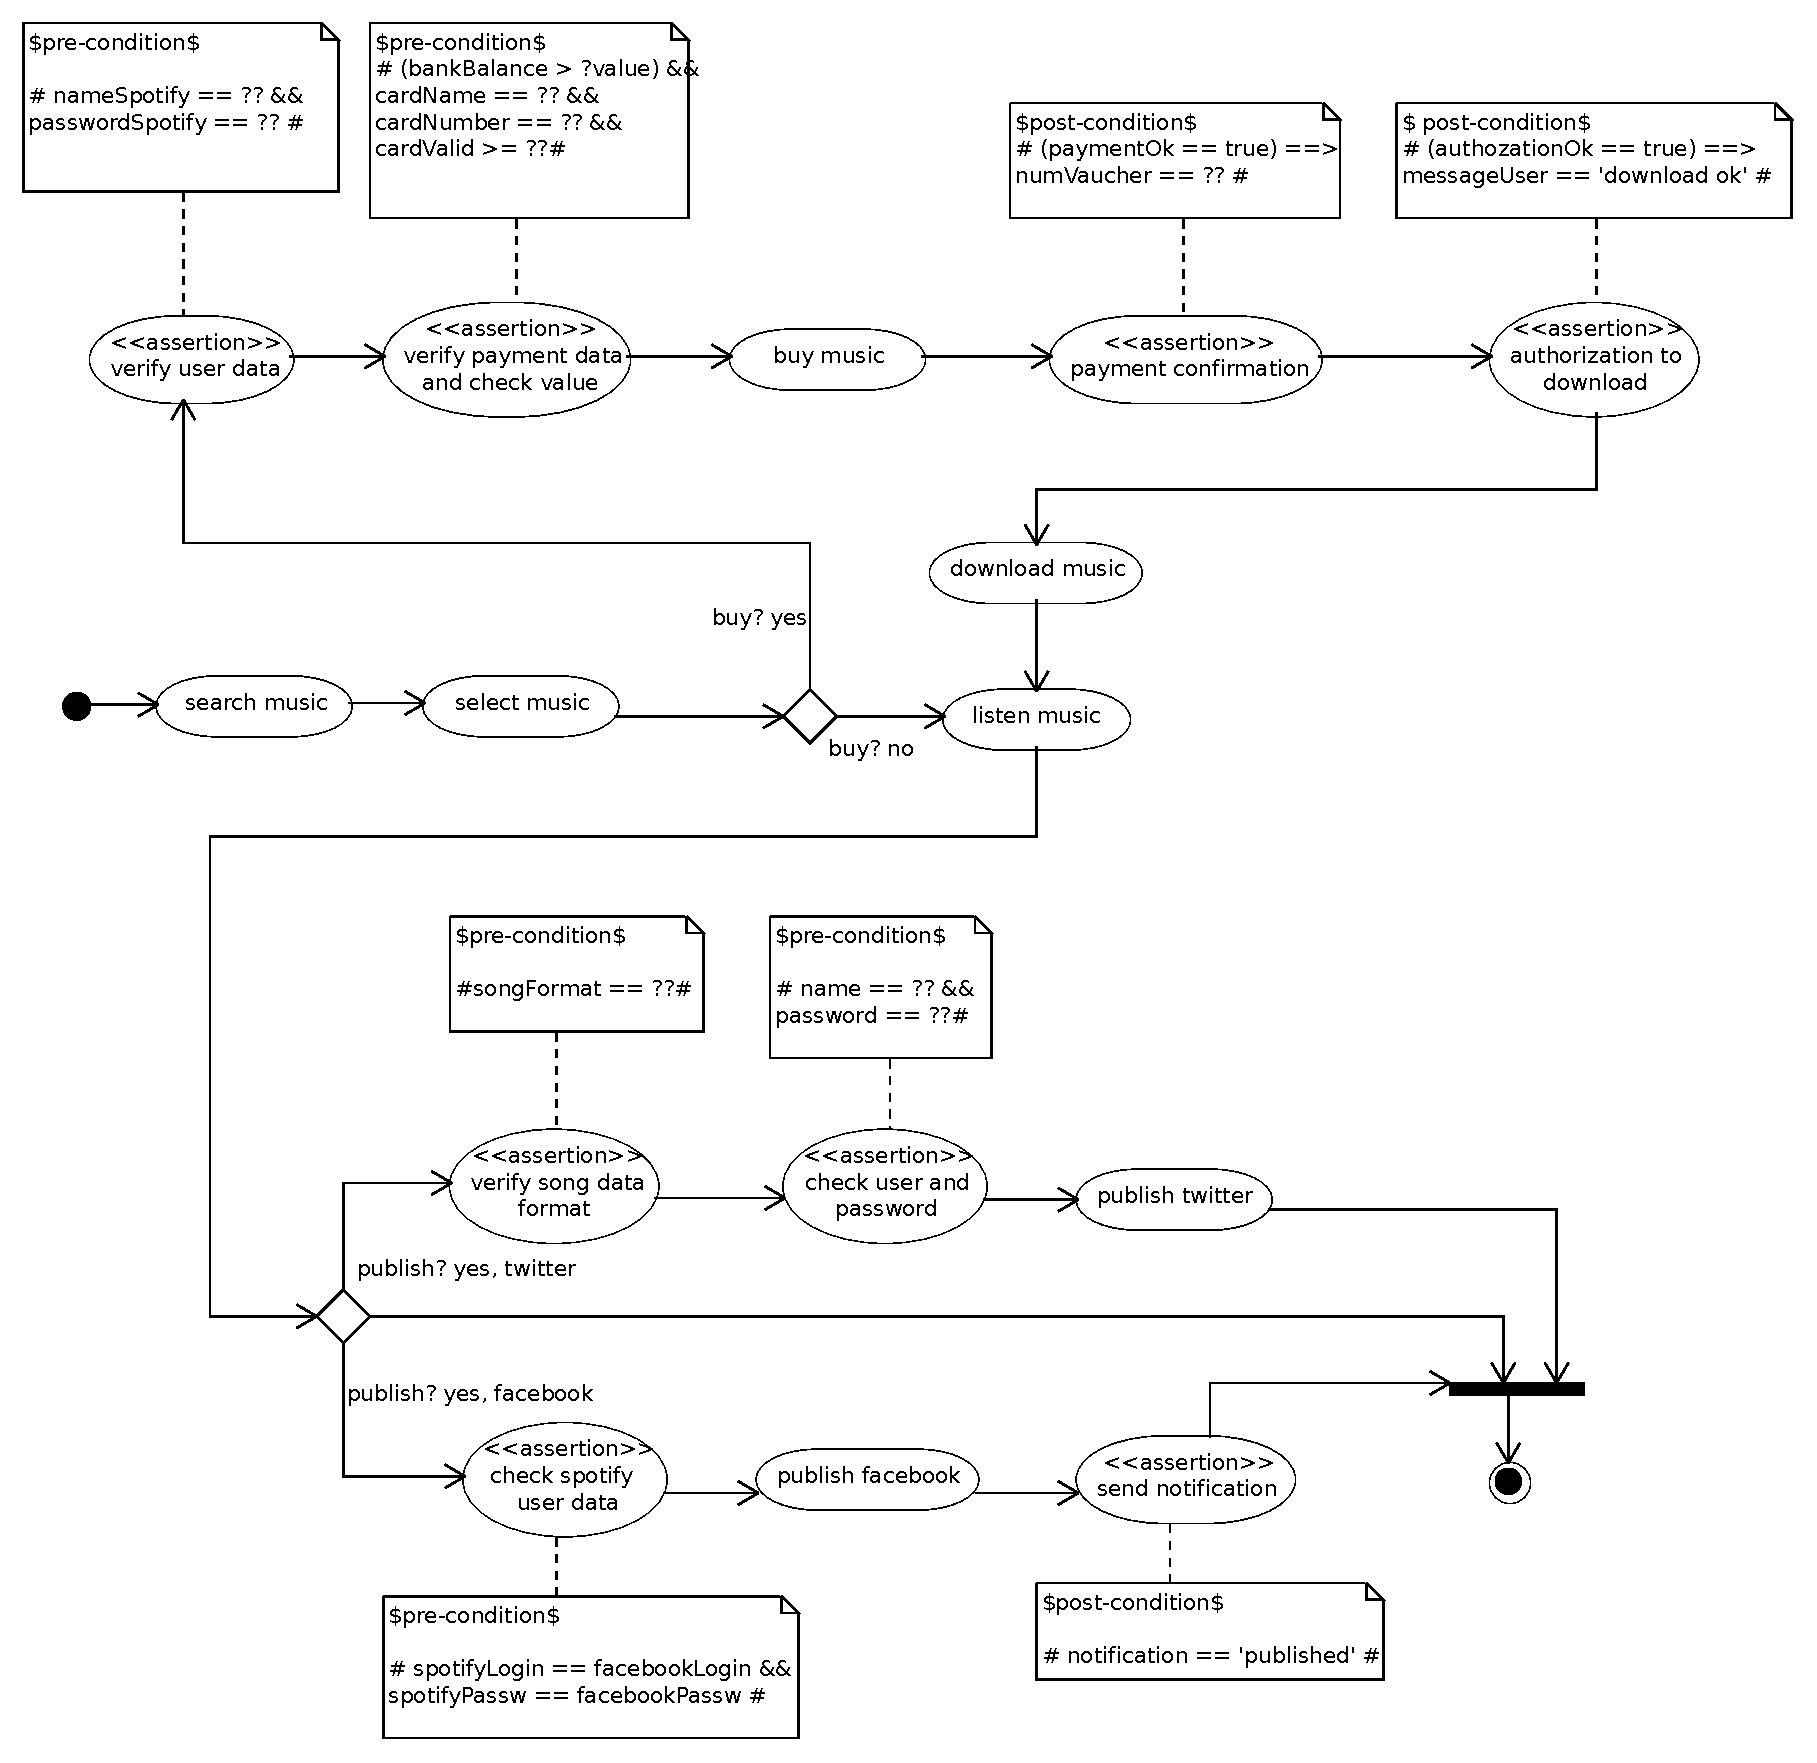
\includegraphics[width=.99\textwidth]{chapters/methodology/figs/piserviceprocess/runningExampleSP_final.pdf}
\caption{\textit{$\pi$-ServiceProcess} - To Publish Music.}
\label{figApp:serviceprocessContract}
\end{figure}
  
\begin{landscape} 
\begin{figure} 
\centering
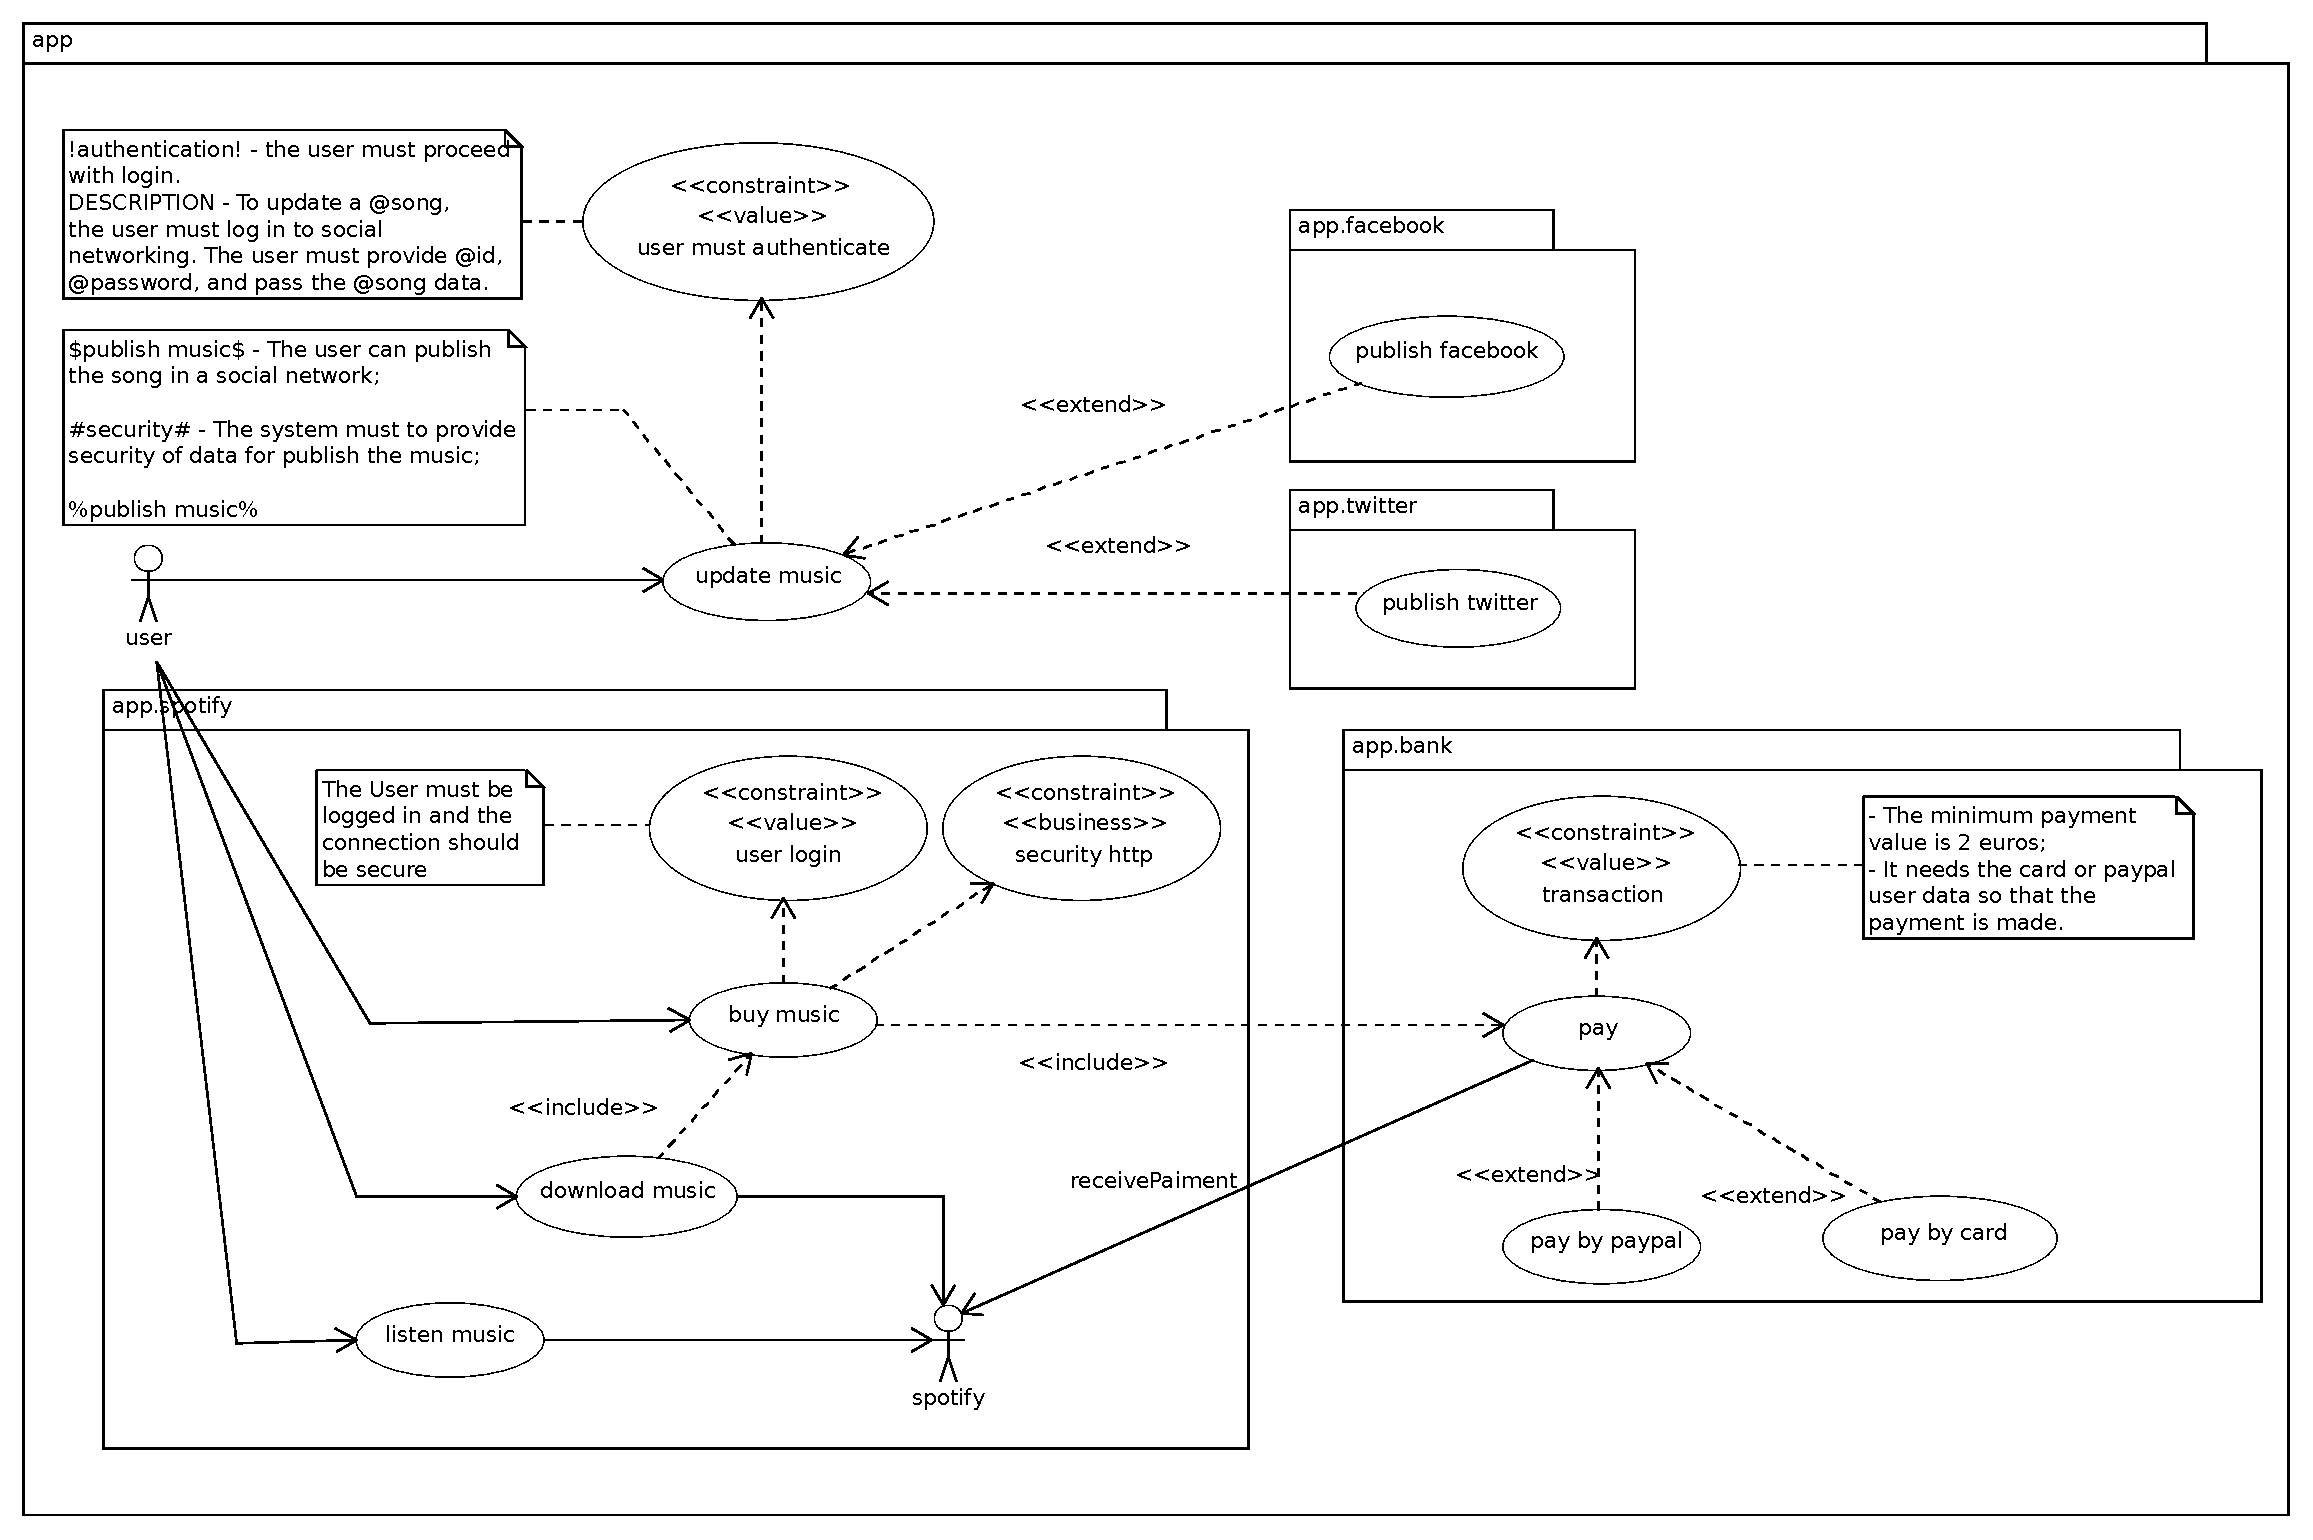
\includegraphics[width=1.4\textwidth]{chapters/state_ofthe_art/figsAppendix/toPublishMusicCompleto.pdf}
\caption{\textit{$\pi$-UseCase} - To Publish Music.}
\label{figApp:toPublishMusicCompleto}
\end{figure} 
\end{landscape}

\begin{landscape}
\begin{figure}[ht!]
\centering
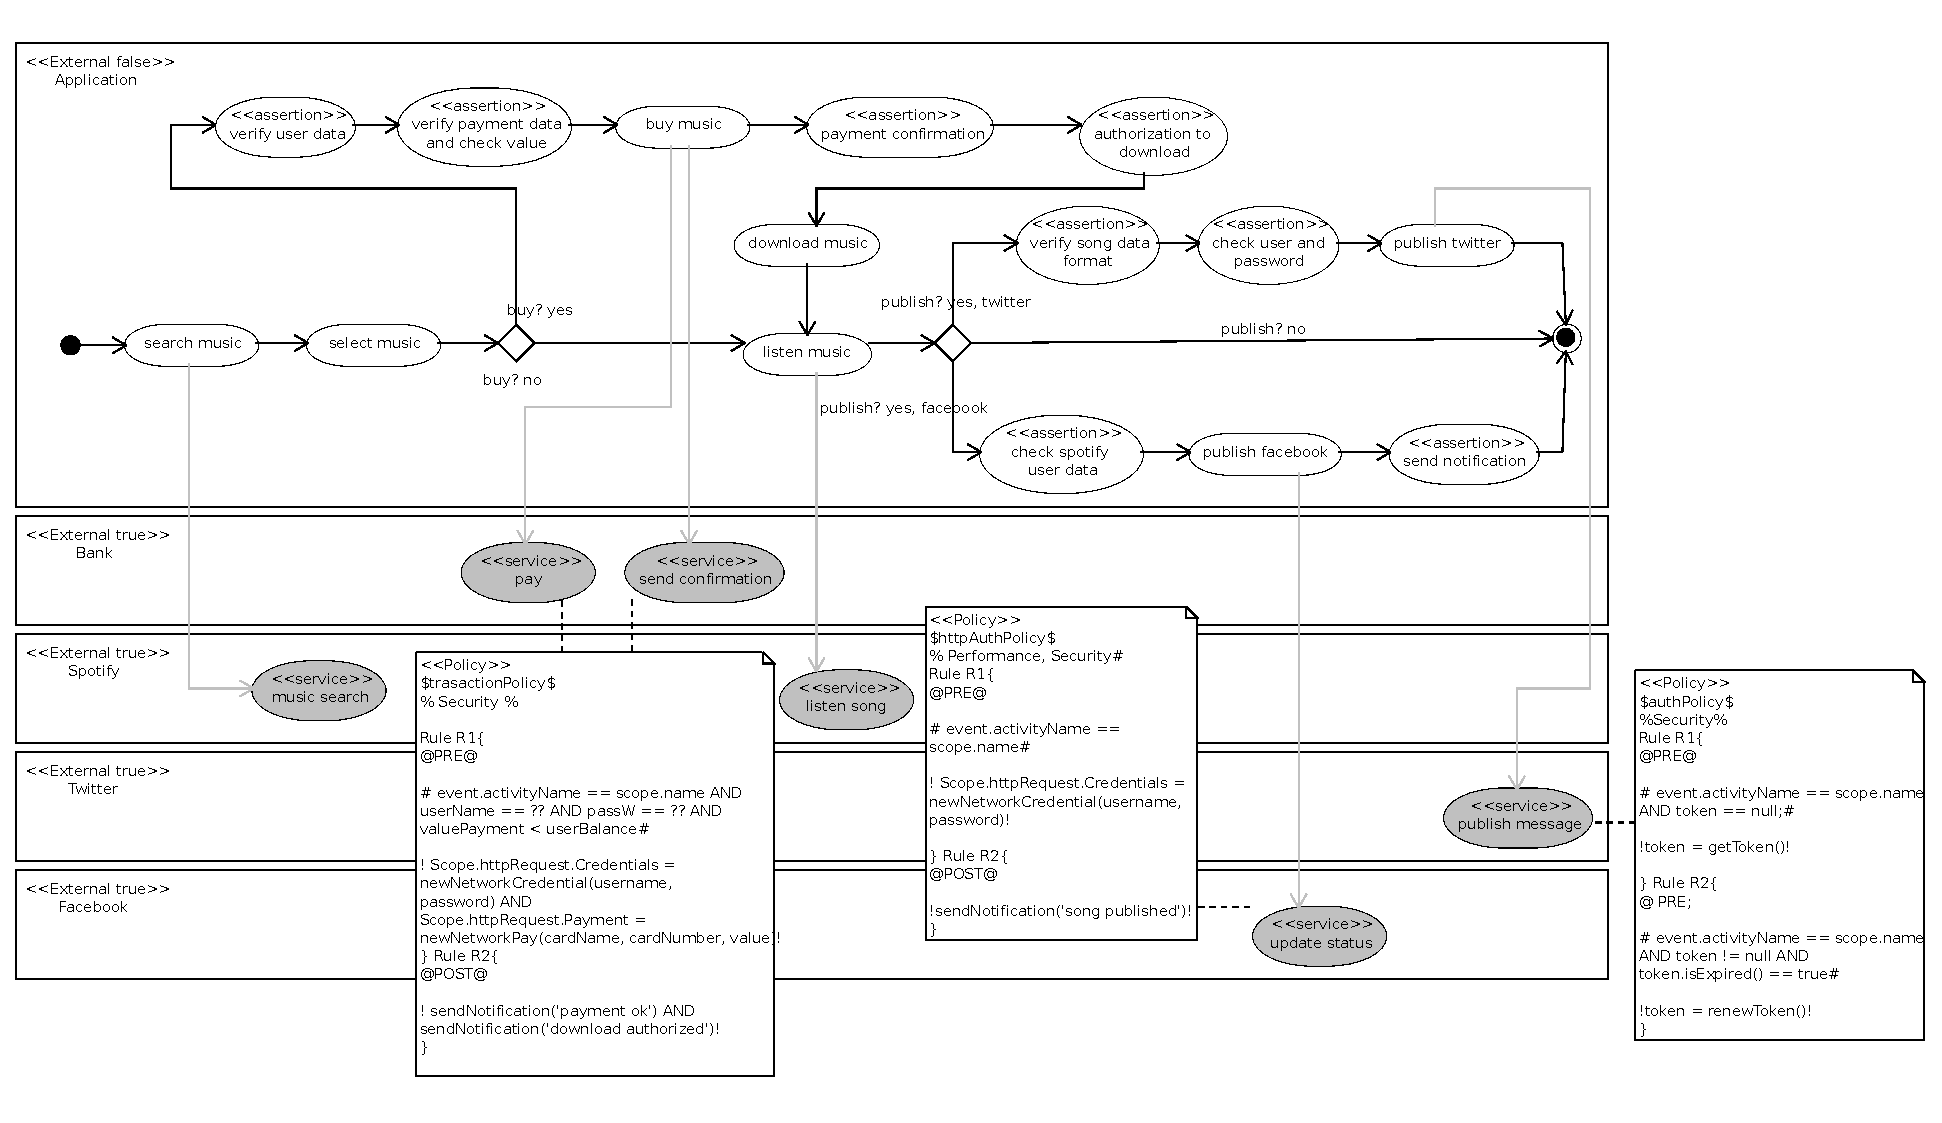
\includegraphics[width=1.44\textwidth]{chapters/methodology/figs/runningExampleServiceComposition.pdf}
\caption{\textit{$\pi$-ServiceComposition} - To Publish Music.}
\label{figApp:servicecompositionPolicy}
\end{figure}
\end{landscape}